% file siminos/froehlich/slice/singul.tex
% $Author$ $Date$

% \section{Slice {\sset}}
%	\label{sec:singul}

If  two patterns are close, their group orbits will be nearly parallel,
$\braket{\groupTan(\ssp)}{\sliceTan{}} \neq 0$, and for a smooth flow the
slice will be transverse to all group orbits of $\ssp$ in an open
neighborhood of the {\template} \slicep.
Looking back at equation \refeq{eq:so2reduced}, we see that the \mslices\
introduces a {\sset} in the \reducedsp. If
$\ssp(\tau)$ is a trajectory in full {\statesp}, then the \reducedsp\
flow $\sspRed(\tau)$ goes through a singularity whenever
\beq
\braket{\groupTan(\sspSing)}{\sliceTan{}}
 =
\braket{\sspSing}{\Lg^2\slicep}
 =0
\,.
\ee{sliceSingl}
Such {\sset s} are purely artifacts of the particular choice of a slice,
and have nothing to do with the particular dynamical system; the
corresponding full \statesp\ trajectory is smooth. Their crossings are
non-generic, but if we consider projections of successive instants of an
ergodic trajectory they can be approached arbitrarily closely. At a
singular instant, the group tangent of a point $\sspRed=\LieEl^{-1} \ssp$
lies in the slice, $\braket{\groupTan(\sspRed)}{\sliceTan{}}$ is zero,
and neither the velocity $\dot{\gSpace}(\tau)$ along the group tangent
nor the velocity in the slice are defined.

At the instant of
coalescence the denominator in \refeq{SF:sliceEas} goes through a simple
pole, and the integrated trajectory within slice jumps. Our next task is
to compute the size of the jump, and describe the behavior of nearby
trajectories.

not generic, but a computational and visualization nuisance

\subsection{Traversing a slice {\sset}}
\label{sec:sliceSing}


%at time $\tau=0$, $\sspSing = \sspRed(0)$.
%The angle $\gSpace^*$ for rotating a point into the slice must satisfy
 %   \PC{Isn't some of this already worked out in \refexam{exam:CLErotAngle}?
  %      You should refer to already derived results, rather than repeating
   %     the same text}
%\bea
%0             &=&
%\braket{\ssp}{\sliceTan{}}\cos(\gSpace^*) +
%\braket{\groupTan_{}(\ssp)}{\sliceTan{}}\sin(\gSpace^*)
%    \continue
%\tan(\gSpace^*) &=&
%-{\braket{\ssp}{\sliceTan{}}}/{\braket{\groupTan_{}(\ssp)}{\sliceTan{}}}
% \,.
%\label{SF:SO2angleRot}
% \refeq{SF:SO2angleRot}
%\eea
%This equation has two solutions
%$\{\sspSing=\LieEl(\gSpace^*)\ssp, \LieEl(\gSpace^*+\pi)\ssp\}$
%unless both $\braket{\sspSing}{\sliceTan{}}$
%and $\braket{\groupTan_{}(\sspSing)}{\sliceTan{}}$ are zero,
%in which case any angle works (this is exactly the situation
%the trajectory is in when it passes through a singularity
%$\ssp^*$).

%Consider $\gSpace(\tau)$ approaching the singularity value
%$\gSpace^*$ as $\tau \rightarrow 0$.
%The trajectory is smooth, so it can be approximated by the linear
%term in the Taylor expansion,
%$
%\ssp(\tau)=\sspSing+\vel^*\tau+O(\tau^2)
%\,,\qquad
%\vel^* = \vel(\sspSing)
%    \,.
%$
%Hence as $\tau \rightarrow 0$,
%\bea
%\tan(\gSpace)
% = -\frac{\braket{\ssp}{\sliceTan{}}}{\braket{\groupTan_{}(\ssp)}{\sliceTan{}}}
%&\rightarrow&
%-\frac{\braket{\sspSing+\vel^*\tau}{\sliceTan{}}}
%{\braket{\Lg(\sspSing+\vel^*\tau)}{\sliceTan{}}}
%    \continue
%\tan(\gSpace^*) &=&
%     -\frac{\braket{\vel^*}{\sliceTan{}}}
%      {\braket{\groupTan_{}(\vel^*)}{\sliceTan{}}}
%\,.
%\label{SF:snglrAngl}
%\eea
%So at the singular point the slice-rotation angle $\gSpace^*$ is computed as in
%\refeq{SF:SO2angleRot}, but using $\vel^*$ rather than $\ssp^*$; as
%$\ssp$ and  $\vel(\ssp)$ rotate rigidly together, that is OK.

%If we add on the restriction $\braket{\groupTan_{}(\ssp)}{\sliceTan{}}$ \refeq{SF:orientedSlice} be nonnegative so that we get a unique representative from each trajectory, then as the trajectory approaches the singularity $\braket{\groupTan_{}(\ssp)}{\sliceTan{}}\approx \tau \braket{\Lg\vel^*}{\sliceTan{}}$. As $\tau$ goes from negative to positive, this expression changes sign, so when the trajectory goes through the slice,
%according to \refdef{def:movingFrame} we must rotate the trajectory by $\pi$ in order for it to satisfy the restriction.


% 2010-12-20 previously {CLEsingpass}{CLEnearsing2}
 \begin{figure}
 \begin{center}
(a)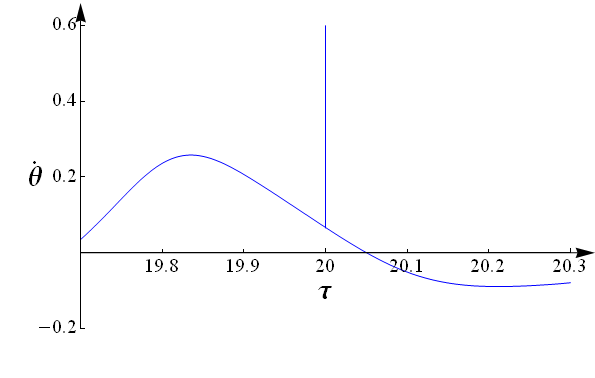
\includegraphics[width=0.45\textwidth]{dthetasing}%
(b)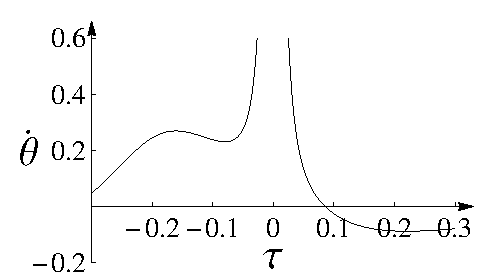
\includegraphics[width=0.45\textwidth]{dthetanearsing}%
 \end{center}
 \caption{\label{fig:dthetasing}
The {\groupVel} $\dot{\gSpace}$ for two \cLf\
\reducedsp\ trajectories in a slice defined by the slice-fixing
point $\slicep=(0.782?,-0.277?,-0.4?,0.12?,0)$:
 (a) As trajectory $\sspRed(\tau)$ passes through the
{\sset} \refeq{sliceSingl}
%$\braket{\groupTan(\sspRed)}{\sliceTan{}}=0$
 at $\sspSing=(-1.22?, ?3.212, -?4.31, ?1.11, ?4)$,
the {\groupVel} diverges
$\dot{\gSpace} \to \infty$ as a Dirac delta function.
(b) The {\groupVel} for a nearby trajectory going
through $\sspSing+\delta \sspRed$,
where $\delta\sspRed=(0.01,0,0,0,0)$.
 }%
 \end{figure}

% 2010-12-20 previously {singpass}%
 \begin{figure}
 \begin{center}
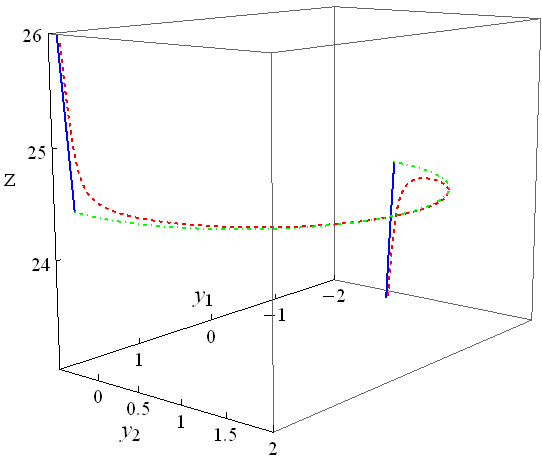
\includegraphics[width=0.45\textwidth]{singpass1}
 \end{center}
 \caption{\label{fig:singpass}
(color online).
Blow-up of the jump in \reffig{fig:Fullspace}\,(b).
(blue/dotted) A trajectory that passes through the singularity point
$\sspSing=(-0.44, 3.23, -0.034, 6.37, 2.34)$ in the slice normal to
$\sliceTan{}=(-0.45, -1.05, 0.3, 0.5, 0.)$.
Note the gap in the trajectory; this corresponds to the jump cause by
passing through the singularity. The red/dashed trajectory has initial
point differing from the blue's by $(0,0,0.1,0,0)$, so it does not pass
through a singularity. The green trajectory is the group orbit of
$\sspSing$ between the two $\gSpace$ that rotate $v(\sspSing)$ in the
slice. Note also how the red/dashed trajectory begins near the
blue/dotted trajectory, closely follows the green trajectory after the
singularity point, reaches the other side of the blue/dotted arc and then
resumes closely following the blue/dotted trajectory.
 }%
 \end{figure}

\reffig{fig:dthetasing}


The {\groupVel} for two \cLf\
\reducedsp\ trajectories in a slice defined by the slice-fixing
point $\slicep=(0.782?,-0.277?,-0.4?,0.12?,0)$.
	\PC{move numerical values of \slicep\ from
	\reffig{fig:dthetasing} and \reffig{fig:singpass} captions
	to formulas in the main text. Explain where they come from}

As a trajectory $\sspRed(\tau)$ passes through the
{\sset} \refeq{sliceSingl}
the {\groupVel} diverges
$\dot{\gSpace} \to \infty$ as a Dirac delta function.

(b) The {\groupVel} for a nearby trajectory going
through $\sspRed+\delta \sspRed$,
where $\delta\sspRed=(0.01,0,0,0,0)$.


\reffig{fig:singpass}


%
% ****** End of file singul.tex ******
